%% LaTeX2e class for student theses
%% sections/evaluation.tex
%% 
%% Karlsruhe Institute of Technology
%% Institute for Program Structures and Data Organization
%% Chair for Software Design and Quality (SDQ)
%%
%% Dr.-Ing. Erik Burger
%% burger@kit.edu
%%
%% Version 1.3.2, 2017-08-
\chapter{Evaluation}
\label{ch:eval}
In this chapter, we evaluate the process to create a case on the basis of the application to the CoCoME system. Also, the created case study is evaluated. Then PCM modeling language is evaluated, if it is possible to express the created case study. At last, the results of the evaluation are discussed to conclude this chapter.
\section{GQM plan}
Three aspects of the thesis are evaluated. First, the applicability of the introduced method, secondly the usability of the created case study for data based privacy analysis and and last but not least to what extent it is possible to model the created case study with PCM. 
%Reicht das als Hinweis ?
 Each evaluation follow a GQM plan \cite{GQM_Intro}, which is shown in \autoref{GQMPlan}. 
\begin{figure}
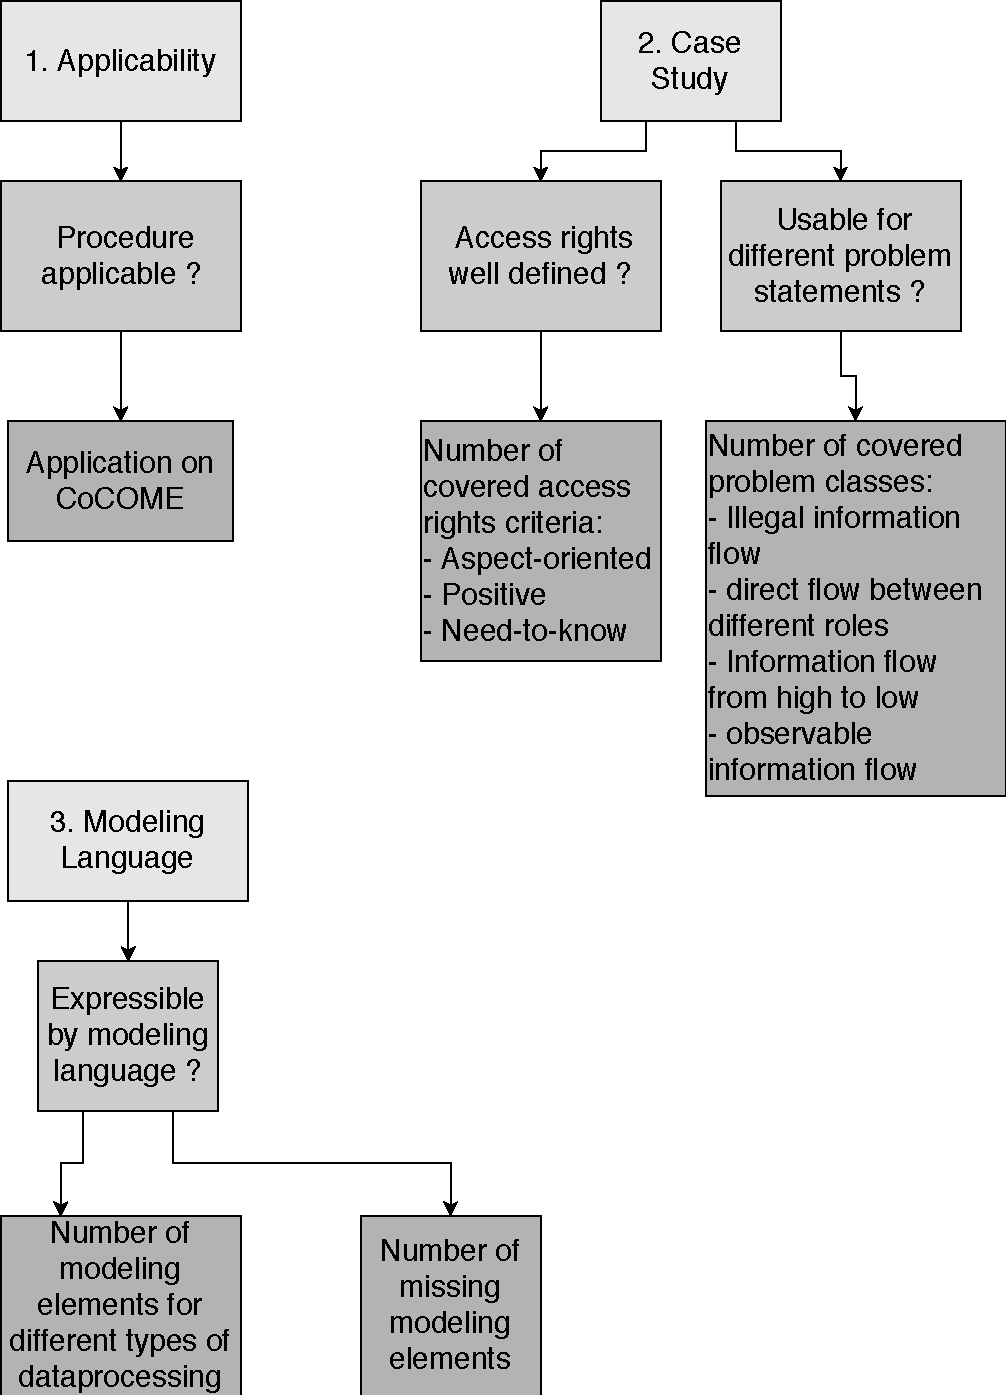
\includegraphics[scale=.8, origin=c ]{logos/OverviewEval.pdf}
\caption{The GQM plan for the three parts of the evaluation. Each part is divided into }01
\label{GQMPlan}
\end{figure}
\section{Applicability of the introduced method}
The first aspect we want to evaluate is applicability of the introduced method for software systems. We check this so the method an be used to create further case studies. 
\subsection{Is the introduced method applicable to a concrete system}
To verify if the goal is achieved, we defined the following question:\\
Is the method applicable for a system that models a PickupShop?\\
Pickupshop in this case means, that orders are placed online and picked up later by the customer.
As a metric for answering the question, we take the successful application of the method to CoCoME. 
\subsubsection{Application to the CoCoME system}
In the chapters \autoref{ch:cocome} and \autoref{casestudysystem}, the application of the method to CoCoME is shown. It is possible to create case study for the CoCoME. We followed the steps described in chapter \nameref{ch:method} and after all the steps were taken we successfully created a case study. The use to carry out data-based data protection analyses is evaluated in  \autoref{usage_DBPA}. In \autoref{casestudysystem} we successfully created a case study for the examined excerpt. Therefore, we concluded that the method is applicable for the reduced system.
\section{Usability of the created case study for data-based privacy analysis}
\label{usage_DBPA}
The next aspect we evaluated the usability of the created case study. A case study is not useful if it does not meet criteria. The criteria ensure that the case study is in a state where it can be used for data-based data privacy analysis. To ensure this, we evaluate two different parts of the case study. First, we evaluate the defined access rights, then the defined data flows. 


\section{Expressiveness of data centric PCM}
The last evaluation aspect of this thesis is to evaluate the chosen modeling language, in this case data-centric PCM. We want to check to what extent PCM is able to add the access rights and data flows in the already existing system model. To allow the extension, Seifermann \cite{MMextension} provided a meta model extension. This meta model extension is the central point of the evaluation. Without the meta model extension, PCM is not able to store data flows and access control rights directly in a system model. 
\subsection{Is the created case study expressible with PCM ?}
A as metric to verify if the, we use the created case study and check if all operations for the different types of data are expressible by PCM. Also we check if elements for types of data processing are missing. The metric is done in a checklist manner. 
\subsubsection{Number of available elements to model the different types of data processing}
First we measure in what current state the operations of the meta model extension are in. We identified five types of data processing that are needed to express the data flows. Currently twelve operations are available in the meta model extension. We measure which operation express the which type of data processing.
\paragraph{Operations relational algebra}
This type of data processing describes the manipulation of database or data requested from databases. The operations for this are available in the meta model. 
\paragraph{I/O- operations}
This type of data processing describes an I/O operation in the data flow, where a user receives data and inputs the same or an other data type in the system. An operation for this is available. 
\paragraph{Transmission data}
This data type describes if component transmit types of data. An operation for this available in the meta model extension. 
\paragraph{Change Access rights}
In the course of a data flow it may happen, that the access right level of a data type changes. For this case an operation in the meta model extension is available. This mostly happens when an operation changes the type of data. This type of processing is closely related to the next one described. 
\paragraph{Alternation of data}
This is a larger type of operations. All in all, this type describes the alternation of data. This includes
creation of data, merging many points in , for example, into list or set. Also the splitting data, like lists, in the different data points. This type of data processing describes the contrasting operation to merging data in collections. 
\subsection{Number of missing elements for the different }
An element for modeling the ACM in the system model is missing.
\section{Discussion}
After all the evaluations are conducted, we discuss the findings. This discussion will be divided into three parts. Each parts covers one of the evaluation aspects shown in \autoref{GQMPlan}.\\
We were able to verify that the method is applicable to a system that models a pickup shop. The method should also be applied to other systems. Possible other systems are flight booking systems, food suppliers, etc. The weakness in this part of the evaluation is that the method has not been applied often enough to different systems to make a statement about its applicability.\\
In the next part, the evaluation results of the access rights and data flows are discussed. First, the defined access rights in the case study. We evaluated based on predefined criteria by Evered and Bögeholz \cite{CaseStudyAndAccessrigths} the access rights. Not all criteria were applicable to the case study, because for some criteria one need running code which is not in the scope of the case study. Other criteria weren't applicable due to time constraints. All in all, as shown in \autoref{eval_AR}, we achieved with our definition of the access rights all three criteria. There is surely some work to be done to allow to check more criteria, like conducting a survey for the criteria clear and concise. For the criteria fundamental and efficient a deployment of CoCoME which includes the access rights is needed. The evaluation of the access rights has to be taken with a grain of salt. Since the access rights depend on the security-relevant data and the roles defined in the system, they must be reevaluated if something has changed.  The evaluation is therefore only a snapshot of the current quality of the access rights. Next, we discuss the evaluation for the different covered information flow classes. We achieved to cover two of the four information flow classes, which is a pretty solid. As we see it, the desirable state is to cover all information flow classes in width and depth. Width means that at least each class is covered by at least one data flow. Depth means that for each class a data flow is defined that is illegal for the class and one that it is not.As shown in \autoref{eval_DF}, we only cover two information flow classes. 
At last we discuss the results for our modeling language PCM. We defined five types of data processing and evaluated whether they are possible to model in PCM. The result is shown in \autoref{eval_MM}. As shown, all types of data processing are modeled. Therefore, we conclude it is be possible to model all created case studies with PCM. But it is not possible to store the ACM in the same model. 
\begin{table}
\begin{tabular}{|c|c|}
\hline 
Access Rights & fulfilled ? \\ 
\hline 
Aspect-oriented & yes \\ 
\hline 
Positive & yes \\ 
\hline 
Need-to-know & yes \\ 
\hline 
\end{tabular} 
\caption{Overview of the evaluation result for the access rights.}
\label{eval_AR}
\end{table}

\begin{table}
\begin{tabular}{|c|c|}
\hline 
Data flow & fulfilled \\ 
\hline 
Illegal information flow & yes \\ 
\hline 
Information flow from high to low & yes \\ 
\hline 
Observable information  flow & no \\ 
\hline 
Direct information flow between roles & no \\ 
\hline 
\end{tabular} 
\caption{Overview over the evaluation result for the data flows.}
\label{eval_DF}
\end{table}
 
\begin{table}
\begin{tabular}{|c|c|}
\hline 
Meta model  & possible ? \\ 
\hline 
relational algebra & yes \\ 
\hline 
I/O operations & yes \\ 
\hline 
Transmission of data & yes \\ 
\hline 
Change of access rights & yes \\ 
\hline 
Alternation of data & yes \\ 
\hline 
ACM in system model & no \\
\hline
\end{tabular} 
\caption{Overview over the results for the evaluation of PCM.}
\label{eval_MM}
\end{table}
To conclude the evaluation, one can say that we introduced an applicable method for a certain typ eof systems to create data flows for a data-based privacy analysis. For the sample case study, we say it is a proof-of-concept, because only two class of information are modeled. The defined access rights are well defined in the current evaluation, but it is imperative to apply the other criteria to get a more complete picture. It must also be said that access rights are relatively volatile, as there is a need to check even small changes in the system. At last, the used modeling language is able to model all types of data processing and is therefore usable for data-based privacy analysis. The only throwback for the modeling language is that the ACM must be stored separately, this may lead to inconsistency and should be fixed soon.
